\subsection{Facade}
\subsubsection{Định nghĩa}
Facade là một mẫu thiết kế (design pattern) thuộc nhóm cấu trúc (structural pattern) trong lập trình hướng đối tượng. Facade Pattern cung cấp cho chúng ta một giao diện chung đơn giản thay cho một nhóm các giao diện có trong một hệ thống con (subsystem). Facade Pattern định nghĩa một giao diện ở cấp độ cao hơn để giúp cho người dùng có thể dễ dàng sử dụng hệ thống con này..
\subsubsection{Cách sử dụng}
Chúng ta sẽ sử dụng Fancade trong trường hợp:
\begin{itemize}
    \item Khi có rất nhiều hệ thống con mà mỗi hệ thống con đó lại có những giao diện riêng lẻ của nó nên rất khó cho việc sử dụng phối hợp.
    \item Khi bạn muốn giảm sự phụ thuộc giữa các thành phần của hệ thống và người sử dụng bên ngoài.
    \item Khi bạn muốn tạo ra một lớp bao bọc (wrapper) để ẩn đi chi tiết bên trong và cung cấp một giao diện đơn giản và rõ ràng.
\end{itemize}
\subsubsection{Cấu trúc}
\begin{itemize}
    \item Thực chất, Facade là gôm tất cả các class cùng loại vào một class để dễ sử dụng.
    \item Có thể có nhiều lớp Facde để phục vụ mục đích giải quyết bài toán.
\end{itemize}
Các thành phần chính:
\begin{itemize}
    \item Một hệ thống các sản phẩm kế thừa phức tạp và các chức năng của nó.
    \item Một Facde class biết được hệ thống nào sẽ đáp ứng yêu cầu nào của người dùng.
    \item Một Additonal Facade được tạo ra để phân lớp giúp Facade đỡ phức tạp.
\end{itemize}
\begin{center}
    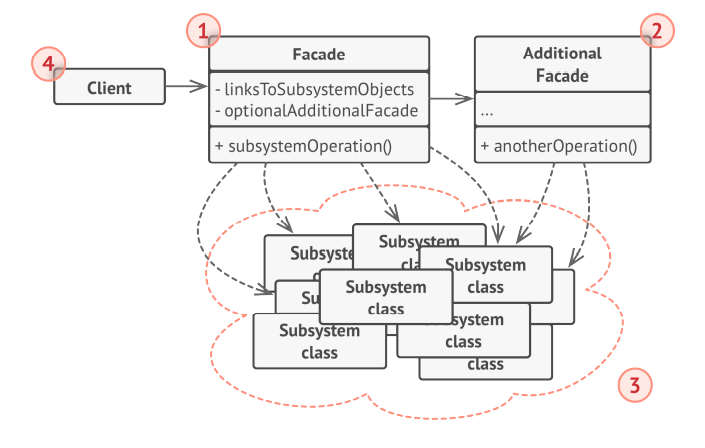
\includegraphics[scale=0.5]{image/structural/facade.png}
\end{center}

\subsubsection{Ưu điểm và Nhược điểm}
Có rất nhiều ưu nhược điểm dễ thấy như sau:\\\\
Ưu điểm:
\begin{itemize}
    \item Ta có thể tách mã nguồn của mình ra khỏi sự phức tạp của hệ thống con.
    \item Có thể đóng gói nhiều hàm được thiết kế không tốt bằng 1 hàm có thiết kế tốt hơn.
    \item Giảm sự phụ thuộc giữa các thành phần của hệ thống, tạo sự tách biệt và khả năng mở rộng cao.
\end{itemize}
Nhược điểm:
\begin{itemize}
    \item Không nên sử dụng quá nhiều lớp Facade với các phương thức phức tạp, vì điều này có thể làm cho giao diện trở nên rườm rà và khó hiểu.
    \item Việc sử dụng Facade cho các hệ thống đơn giản, ko quá phức tạp trở nên dư thừa.
\end{itemize}

\subsubsection{Code Example}
\begin{itemize}
    \item Có 3 loại hình là hình chữ nhật, hình tròn, hình tam giác. Mỗi hình có 2 phương thức là vẽ và xóa.
    \item Có 1 ShapeFacade gom cả 3 hình này vào thành thuộc tính và có 3x2 phương thức là 6 để vẽ và xóa cho mỗi loại hình.
\end{itemize}
\begin{lstlisting}
#include <iostream>

// Rectangle
class Rectangle {
public:
    void draw() {
        std::cout << "Draw rectangle" << std::endl;
    }

    void erase() {
        std::cout << "Erase rectangle" << std::endl;
    }
};

// Circle
class Circle {
public:
    void draw() {
        std::cout << "Draw circle" << std::endl;
    }

    void erase() {
        std::cout << "Erase circle" << std::endl;
    }
};

// Triangle
class Triangle {
public:
    void draw() {
        std::cout << "Draw triangle" << std::endl;
    }

    void erase() {
        std::cout << "Erase triangle" << std::endl;
    }
};

// Facade
class ShapeFacade {
private:
    Rectangle rectangle;
    Circle circle;
    Triangle triangle;

public:
    void drawRectangle() {
        rectangle.draw();
    }

    void eraseRectangle() {
        rectangle.erase();
    }

    void drawCircle() {
        circle.draw();
    }

    void eraseCircle() {
        circle.erase();
    }

    void drawTriangle() {
        triangle.draw();
    }

    void eraseTriangle() {
        triangle.erase();
    }
};

int main() {
    ShapeFacade facade;

    facade.drawRectangle();
    facade.eraseRectangle();

    facade.drawCircle();
    facade.eraseCircle();

    facade.drawTriangle();
    facade.eraseTriangle();

    return 0;
}


\end{lstlisting}
Ở hàm main, ta gọi facade và kêu tất cả các hàm có trong facade.\\
\newline
\textbf{Kết quả:}
\begin{lstlisting}
Draw rectangle
Erase rectangle
Draw circle
Erase circle
Draw triangle
Erase triangle
\end{lstlisting}
\subsubsection{Các Pattern liên quan}
\begin{itemize}
    \item Facade khi kết hợp với Abstract Factory có thể ẩn đi hệ thống được sử dụng để gọi ra sản phẩm.
    \item Adapter và Facade khác nhau ở chỗ Adapter sử dụng mã nguồn này thay vì mã nguồn kia còn Facade gôm hết tất cả lại.
    \item Các đối tượng Facade có thể là Singleton vì nó bao gồm toàn bộ các Subsystem.
    \item Vì nó quá lớn nên ta có thể áp dụng Flyweight để làm giảm bộ nhớ nó cần phải trong Ram.
    \item Mediator có công việc tổ chức sự hợp tác giữa các lớp với nhau giống với Facde.
    \item Proxy là một phương thức đệm ngoài Đối tượng chính cũng giống như Facade vậy.
\end{itemize}
